%

\begin{abstract}
%

%


Off-Policy Evaluation (OPE) in contextual bandits is crucial for assessing new policies using existing data without costly experimentation. However, current OPE methods, such as Inverse Probability Weighting (IPW) and Doubly Robust (DR) estimators, suffer from high variance, particularly in cases of low overlap between target and behavior policies or large action and context spaces. In this paper, we introduce a new OPE estimator for contextual bandits, the Marginal Ratio (MR) estimator, which focuses on the shift in the marginal distribution of outcomes $Y$ instead of the policies themselves. Through rigorous theoretical analysis, we demonstrate the benefits of the MR estimator compared to conventional methods like IPW and DR in terms of variance reduction. Additionally, we establish a connection between the MR estimator and the state-of-the-art Marginalized Inverse Propensity Score (MIPS) estimator, proving that MR achieves lower variance among a generalized family of MIPS estimators. We further illustrate the utility of the MR estimator in causal inference settings, where it exhibits enhanced performance in estimating Average Treatment Effects (ATE). Our experiments on synthetic and real-world datasets corroborate our theoretical findings and highlight the practical advantages of the MR estimator in OPE for contextual bandits. 
\end{abstract}
%
%
\documentclass[../main.tex]{subfiles}
\graphicspath{{../images/}}
\makeatletter
\def\input@path{{../images/}}
\makeatother
\begin{document}
\section{Introduction}
\begin{figure}
\centering
\begin{tikzpicture}
\node[inner sep=0pt] (ws) at (0, 0) {
\includegraphics[height=.4\textwidth, trim={10cm 0 10cm 0},clip]{world_space.png}};
\node[inner sep=0pt] (cs) at (6,0) {\includegraphics[height=.4\textwidth, trim={10cm 1cm 10cm 4cm},clip]{conf_space.png}};
\end{tikzpicture}
\vspace{-5pt}
\label{fig:pbrm_intro}
\caption{\textbf{Left}: Shows world space obstacles as grey spheres. Robots start and goal configuration is colored red and green, respectively. Configurations along the computed path are colored transparent blue. \textbf{Right:} Mapped world space scenario to configuration space. Obstacle region is the grey mesh. Red spheres are collision-free regions computed by the neural SCDF. The optimized shortest path in the convex corridor is the blue curve.}
\vspace{-25pt}
\end{figure}
Motion planning is the problem of finding a collision-free trajectory that connects a given start and goal configuration. The planning takes place in the configuration space of the robot. For single body robots, like mobile robots or drones, the configuration space and the world space are usually the same. This simplifies the planning, since explicit obstacle representations are available which enables geometrical tools like separating hyperplanes, smallest distance to obstacles etc., to be used when designing motion planning algorithms. For multi-body robots like manipulators, the situation is completely different. The world space obstacles are usually mapped to non-convex regions, and to make the problem even harder, the mapping is usually not known. Forming explicit representations of the obstacle region in the configuration space is usually too expensive or intractable. Despite all of this, sampling based planners are used with great success, which mainly is due to their use of implicit representations of the obstacle region. The basic idea is to construct a graph in the configuration space that covers and connects the collision-free region. From this graph, a path can be extracted that connects a given start and goal configuration. The approach is computationally expensive, since the graph is constructed with the smallest geometrical building block available, points, which represents a collision-check. Furthermore, the extracted paths from the graph are non-smooth and jagged due to the stochastic nature of the approach. This adds an additional post-processing step to the process, where the paths are shortcutted and smoothened, before the path can be used for tracking. Clearly a lot of time is invested to form this graph and produce smooth paths. Thus, if the obstacles start to move, then all of this work is done in no use, since all points that make up this graph need to be re-verified, which is simply too time consuming to be done in real time.
\\\\
In this work, we want to address the existing drawbacks of the sampling based planners. Our main contribution is an improved motion planner where each vertex in the graph covers a collision-free region in the form of a sphere instead of a point and where the edges are formed with neighboring intersecting spheres. This representation has the advantage of instead of returning piecewise linear paths, returning a sequence of overlapping spheres, i.e. a convex corridor, that connects a given start and goal configuration, illustrated in Figure \ref{fig:pbrm_intro}. This convex corridor allows us to use convex optimization to produce smooth trajectories, instead of computationally expensive post-processing methods. The representation further allows us to estimate the coverage of the collision-free space, which gives us awareness and feedback in the offline roadmap construction phase. Finally, our representation is simple to adapt to moving obstacles, simply requery for the new radii and recheck for intersections. 
\\\\
The spherical collision-free regions are formed using a signed distance function (SDF), which is a function that returns the smallest distance from an arbitrary point to the boundary of an obstacle. As the name implies, the distance is signed, thus if the point is inside the obstacle it is negative otherwise positive. If the distance is positive, a sphere with radius equal to the distance is guaranteed to cover a collision-free region. Using an SDF in motion planning is not new, but what is novel about our approach is that we express the distance in the configuration space instead of the world space and by doing so allows us to form these convex collision-free regions. We refer to the resulting SDF as a signed configuration distance function (SCDF). Computing an SCDF analytically is non-trivial, our approach is therefore to parameterize the SCDF with a deep neural network and learn the mapping by supervised learning. Our resulting neural SCDF can compute distances for different parameter values of obstacle shapes and we also show how multiple distances can be combined, thus making our approach flexible.
\section{Related work}
Motion planning algorithms can roughly be divided into three families, grid-based, sampling based and optimization based methods. Grid-based methods (GBM) discretize the planning space from which a graph is then compiled. A standard search method is A$^\star$ \citep{a_star}, which is classified as an \textit{informed} search method, since it employs a heuristic function to speed up the search. A$^\star$ guarantees to return an optimal path at the level of discretization used. GBMs usually discretize the planning space by a regular lattice and this limits the GBMs to problems with low dimensionality due to the curse of dimensionality. Thus, GBMs are usually limited to single-body robots where the degrees of freedom (DOF) are low. To overcome the inherent scaling problem with the GBMs, stochastic methods are usually used for multi-body robots. These methods are termed as sampling-based methods (SBM) and core members within this family are the rapidly-exploring random trees (RRT) \citep{rrt} and the probabilistic roadmap (PRM) \citep{prm}. RRT grows a tree from the start configuration and explores the collision-free region in a rapid way until it is able to connect to the goal region. RRT is usually improved by bi-directional planning \citep{rrt_connect}, i.e. an additional tree is grown from the goal configuration and the trees are tested for connection after any tree has been expanded. RRT is a single-query method, thus it searches for a path from scratch each time it is queried. Contrary to this, PRM is a multi-query method, which solves for multiple queries without starting from scratch. PRM does this by creating a roadmap (graph) that covers the collision-free space as an offline step. The graph is then used to solve for multiple queries. PRMs are used in cases where the environment does not change since the extra offline step is too computationally costly and needs to be re-done if the environment is changed. In our work, we address this inherent issue by using a different roadmap representation. Our vertices in the graph cover a collision-free region in the form of spheres and we form the edges by checking for intersecting spheres. If something in the environment changes, we recompute the spheres radii and recheck the intersections, without relying on collision detection. We use a trained neural network to compute the sphere radius, therefore querying for the radius can be done fast, hence our representation enables the PRM for dynamic environments.
\\\\
In the recent decades, optimization based methods (OBM) \citep{chomp, schulman, itomp, stomp} have been introduced as an alternative to SBM for multi-body robots. Like the SBM, the OBMs scale well to higher dimensional problems and produce smoother motion. It is common to use a SDF in the optimization since it is a smooth function, thus enabling gradient-based methods. However, the standard way of expressing the SDF is in world space. The distance therefore needs to be mapped to the configuration space by the forward kinematics. This mapping makes the optimization problem a non-linear program (NLP), which is computationally expensive to solve. Recently, a different approach has been proposed. In \cite{mp_gcs} motion planning is formulated as a convex optimization problem by using the graph of convex sets framework \citep{gcs}. The underlying idea is to decompose the collision-free space into intersecting convex sets from which a convex optimization problem is formulated. In cases where an explicit representation of the obstacles in the configuration space exists, like for single-body robots, creating collision-free convex regions can be done fast \citep{iris}. For multi-body robots, this is non-trivial. Existing work does this successfully \citep{iris_nlp, iris_c} by an optimization based approach, but the methods are still too time consuming to be used in the presence of moving obstacles. Our approach is instead to use deep learning to learn an SDF expressed in the configuration space. With this, we can query for shortest distances to the collision boundary, which allows us to expand spherical regions which are collision-free. Our approach is fast and therefore enables our suggested roadmap planner to be used in dynamic environments.
\\\\
Recent research has focused on learning collision detection \citep{fk_kernel_distance, diffco, graphdistnet} by predicting the signed distance between the robot links and the surrounding obstacles in the world space. The learned SDF is used in trajectory optimization but since the distance is expressed in the world space, the problem becomes an NLP and therefore takes a long time to solve. We take a novel approach and suggest to instead express the signed distance in the configuration space. This allows us to improve the PRM at the same time as it enables convex optimization for trajectory optimization, which runs faster and is more reliable than NLP solvers. In \cite{cspf} a learned signed distance function in the configuration space is proposed similar to our approach. However, their approach is restricted to point cloud representations, while we propose to represent the obstacles as parameterized geometric shapes, e.g. spheres. Furthermore, we also show how to use our learned SCDF to improve an existing roadmap planner.
\section{Problem formulation}
A robot is located in the world space, $\W \subset \R^3 $. The unique location of the robot is given by its configuration $\q \in \C$, where $\C$ is the configuration space. The set of points covered by the robots bodies at a certain configuration is expressed as $\B(\q) \subset \W$. The robot is surrounded by $\NrObst$ obstacles $\O = \bigcup_{i=1}^{\NrObst} \O_i$, where  $\O_i \subset \W$. The representation of the obstacle in the configuration space is the set $\C\O_i = \{\q \in \C \: |\: \B(\q) \cap \O_i \neq \emptyset \}$. The obstacle space is formed as $\Co = \bigcup_{i=1}^{\NrObst} \C \O_i$. The complement is referred to as the free space, $\Cf = \C \setminus \Co$. The path planning problem is a tuple, ($\Cf$, $\qStart$, $\qGoal$), where we want to connect a query pair, consisting of a start, $\qStart$, and goal configuration, $\qGoal$, with a geometric path, $\q(s): [0, 1] \mapsto \Cf$, such that $\q(0)=\qStart$ and $\q(1)=\qGoal$, or report correctly when such a path does not exist.
\end{document}


\section{Background}
\subsection{Setup and Notation} \label{sec:setup_notation}
We consider the standard contextual bandit setting. Let $X\in\Xspace$ be a context vector (e.g., user features), $A\in \Aspace$ denote an action (e.g., recommended website to the user), and $Y\in \Yspace$ denote a scalar reward or outcome (e.g., whether the user clicks on the website). The outcome and context are sampled from unknown probability distributions $p(y\mid x, a)$ and $p(x)$ respectively. Let $\D\coloneqq \{(x_i, a_i, y_i)\}_{i=1}^n$ be a historically logged dataset with $n$ observations, generated by a (possibly unknown) \emph{behaviour policy} $\beh(a\mid x)$.
Specifically, $\D$ consists of i.i.d. samples from the joint density under\textit{ behaviour policy},
\begin{align}
    \pbeh(x, a, y) \coloneqq p(y\mid x, a)\, \textcolor{blue}{\beh(a\mid x)}\,p(x). \label{eq:behav-joint-factorisation}
\end{align}
We denote the joint density of $(X, A, Y)$ under the \textit{target policy} as
\begin{align}
    \ptar(x, a, y) \coloneqq p(y\mid x, a)\, \textcolor{red}{\tar(a\mid x)}\,p(x). \label{eq:tar-joint-factorisation}
\end{align}

Moreover, we use $\pbeh(y)$ to denote the marginal density of $Y$ under the behaviour policy, 
\begin{align*}
    \pbeh(y) &= \int_{\Aspace \times \Xspace} \pbeh(x, a, y)\, \mathrm{d}a \, \mathrm{d}x,
\end{align*}
and likewise for the target policy $\tar$. Similarly, we use $\Ebeh$ and $\Etar$ to denote the expectations under the joint densities $\pbeh(x, a, y)$ and $\ptar(x, a, y)$ respectively.


\myparagraph{Off-policy evaluation (OPE)}
The main objective of OPE is to estimate the expectation of the outcome $Y$ under a given target policy $\tar$, i.e., $\Etar [Y]$, using only the logged data $\D$.
%
%
%


%
%
%
%
%
%
%
%
%
%
%
%

%
%
%
%
%

Throughout this work, we assume that the support of the target policy $\tar$ is included in the support of the behaviour policy $\beh$. This is to ensure that importance sampling yields unbiased off-policy estimators, and is satisfied for exploratory behaviour policies such as the $\epsilon$-greedy policies. 
\begin{assumption}[Support]
    For any $x \in \Xspace, a \in \Aspace$,  $\tar(a\mid x) >0 \implies \beh(a\mid x) >0$. 
\end{assumption}
%
 

\subsection{Existing off-policy evaluation methodologies}
Next, we will present some of the most commonly used OPE estimators before outlining the limitations of these methodologies. This motivates our proposal of an alternative OPE estimator. 

The value of the target policy can be expressed as the expectation of outcome $Y$ under the target data distribution $\ptar(x, a, y)$.
%
%
%
%
However in most cases, we do not have access to samples from this target distribution and hence we have to resort to importance sampling methods.
\paragraph{Inverse Probability Weighting (IPW) estimator}
One way to compute the target policy value, $\Etar[Y]$, when only given data generated from $\pbeh(x, a, y)$ is to rewrite the policy value as follows:
%

\begin{small}
\begin{align*}
    \Etarred[Y] =
    \int y \, \ptar(x, a, y) \,\mathrm{d}y \, \mathrm{d}a\, \mathrm{d}x   =
    \int y \, \underbrace{\frac{\ptar(x, a, y)}{\pbeh(x, a, y)}}_{\rho(a,x)}\, \pbeh(x, a, y) \,\mathrm{d}y \, \mathrm{d}a\, \mathrm{d}x =
    %
    \Ebehblue\left[Y\,\rho(A, X)\right],
\end{align*}
\end{small} 
where 
$
\rho(a, x) \coloneqq \frac{\ptar(x, a, y)}{\pbeh(x, a, y)} = \frac{\tar(a|x)}{\beh(a|x)}
$, given the factorizations in Eqns. \eqref{eq:behav-joint-factorisation} and \eqref{eq:tar-joint-factorisation}.
This leads to the commonly used \emph{Inverse Probability Weighting (IPW)} \citep{horvitz1952generalization} estimator:
\[
\thetaipw \coloneqq \frac{1}{n}\sum_{i=1}^n \rho(a_i, x_i)\,y_i.
\]
When the behaviour policy is known, IPW is an unbiased and consistent estimator. However, it can suffer from high variance, especially as the overlap between the behaviour and target policies decreases. 

\myparagraph{Doubly Robust (DR) estimator} 
To alleviate the high variance of IPW, \cite{dudik2014doubly} proposed a \emph{Doubly Robust (DR)} estimator for OPE. 
DR uses an estimate of the conditional mean $\hat{\mu}(a, x) \approx\E[Y\mid X=x, A=a]$ (\emph{outcome model}), as a control variate to decrease the variance of IPW. It is also doubly robust in that it yields accurate value estimates if either the importance weights $\rho(a, x)$ or the outcome model $\hat{\mu}(a, x)$ is well estimated \citep{dudik2014doubly, jiang2016doubly}. 
The DR estimator for $\Etar[Y]$ can be written as follows:
\[
\thetadr = \frac{1}{n} \sum_{i=1}^n \rho(a_i, x_i)\,(y_i - \hat{\mu}(a_i, x_i)) + \hat{\eta}(\tar),
%
\]
where
$
\hat{\eta}(\tar) = \frac{1}{n} \sum_{i=1}^n \sum_{a'\in \Aspace} \hat{\mu}(a', x_i) \tar(a'\mid x_i) \approx \E_{\tar}[\hat{\mu}(A, X)]$. Here, $\hat{\eta}(\tar)$ is referred to as the Direct Method (DM) as it uses $\hat{\mu}(a, x)$ directly to estimate target policy value. 

\subsection{Limitation of existing methodologies} 
To estimate the value of the target policy $\tar$, the existing methodologies consider the shift in the joint distribution of $(X, A, Y)$  as a result of the policy shift (by weighting samples by policy ratios). As we show in Section \ref{subsec:comparison}, considering the joint shift can lead to inefficient policy evaluation and high variance especially as the policy shift increases \citep{li2018addressing}.
Since our goal is to estimate $\Etar[Y]$, we will show in the next section that considering only the shift in the marginal distribution of the outcomes $Y$ from $\pbeh(Y)$ to $\ptar(Y)$, leads to a more efficient OPE methodology compared to existing approaches.

To better comprehend why only considering the shift in the marginal distribution is advantageous, let us examine an extreme example where we assume that $Y \indep A \mid X$, i.e., the outcome $Y$ for a user $X$ is independent of the action $A$ taken. In this specific instance, $\Etar[Y] = \Ebeh[Y] \approx 1/n\sum_{i=1}^n y_i,$ indicating that an unweighted empirical mean serves as a suitable unbiased estimator of $\Etar[Y]$. However, IPW and DR estimators use policy ratios $\rho(a, x)  = \frac{\tar(a \mid x)}{\beh(a \mid x)}$ as importance weights. In case of large policy shifts, these ratios may vary significantly, leading to high variance in IPW and DR.

In this particular example, the shift in policies is inconsequential as it does not impact the distribution of outcomes $Y$. Hence, IPW and DR estimators introduce additional variance due to the policy ratios when they are not actually required. This limitation is not exclusive to this special case; in general, methodologies like IPW and DR exhibit high variance when there is low overlap between target and behavior policies \citep{li2018addressing} even if the resulting shift in marginals of the outcome $Y$ is not significant.
%

Therefore, we propose the \emph{Marginal Ratio (MR)} OPE estimator for contextual bandits in the subsequent section, which circumvents these issues by focusing on the shift in the marginal distribution of the outcomes $Y$. Additionally, we provide extensive theoretical insights on the comparison of MR to existing state-of-the-art methods, such as IPW and DR.

%
%

%

%

%






%
%
%
%

\section{Marginal Ratio (MR) estimator}
 
%
%
Our method's key insight involves weighting outcomes by the marginal density ratio of outcome $Y$:
\begin{align*}
\Etarred[Y] &= \int_{\Yspace} y \, \ptar(y)\, \mathrm{d}y = \int_\Yspace y\, \frac{\ptar(y)}{\pbeh(y)} \, \pbeh(y) \, \mathrm{d}y = \Ebehblue\left[Y\, w(Y) \right],
\end{align*}
where 
$
w(y) \coloneqq \frac{\ptar(y)}{\pbeh(y)}.
$
This leads to the Marginal Ratio OPE estimator:
\begin{align*}
    \thetamr \coloneqq \frac{1}{n}\sum_{i=1}^n w(y_i) \, y_i.
\end{align*}

In Section \ref{subsec:comparison} we prove that by only considering the shift in the marginal distribution of outcomes, the MR estimator achieves a lower variance than the standard OPE methods. In fact, this estimator does not depend on the shift between target and behaviour policies directly. Instead, it depends on the shift between the marginals $\pbeh(y)$ and $\ptar(y)$.
%
%
%
%
%

\myparagraph{Estimation of $w(y)$} When the weights $w(y)$ are known exactly, the MR estimator is unbiased and consistent. However, in practice the weights $w(y)$ are often not known and must be estimated using the logged data $\D$. Here, we outline an efficient way to estimate $w(y)$ by first representing it as a conditional expectation, which can subsequently be expressed as the solution to a regression problem.
%
%
%
%
%
%
%
\begin{lemma}\label{lemma:weights-est}
Let $w(y)=\frac{\ptar(y)}{\pbeh(y)}$ and $\rho(a, x) = \frac{\tar(a\mid x)}{\beh(a\mid x)}$, then $w(y) = \Ebeh\left[ \rho(A, X) \mid \,Y=y \right]$, and,
%
%
%
%
\begin{align}
 w = \arg\min_{f} \, \Ebeh \left[(\rho(A, X)-f(Y))^2\right]. \label{eq:weights-obj-main}
\end{align}
\end{lemma}
%
Lemma \ref{lemma:weights-est} allows us to approximate $w(y)$ using a parametric family $\{f_\phi: \mathbb{R}\rightarrow \mathbb{R} \mid \phi \in \Phi\}$ (e.g.\ neural networks) and defining $\hat{w}(y)\coloneqq f_{\phi^*}(y)$, where $\phi^*$ solves the regression problem in Eq. \eqref{eq:weights-obj-main}. 

%
%
%

%
%
%
%
%
%
%
%
%
%

%
%
%

Note that MR can also be estimated alternatively by directly estimating $h(y) \coloneqq w(y)\,y$ 
%
using a similar regression technique as above and computing $\thetamr = 1/n \sum_{i=1}^n h(y_i)$. We include additional details along with empirical comparisons in Appendix \ref{sec:alt-estimation-method}. 
%

\begin{comment}
\subsubsection{Alternative estimation method}\label{sec:alt-estimation-method}
When estimating the MR estimator, we can alternatively estimate $h(y) \coloneqq y\,w(y)$ using 
\begin{align*}
    h = \arg\min_{f} \, \Ebeh \Bigg(Y\,\frac{\tar(A|X)}{\beh (A|X)}-f(Y)\Bigg)^2.
\end{align*}
Subsequently, the MR estimator can be written as:
\[
\thetamr = \frac{1}{n}\sum_{i=1}^n h(y_i).
\]
\paragraph{Remark}
These methods outline two different methodologies of estimating MR. In general, it is difficult to say which of the two methods will perform better. Intuitively speaking, in cases where the behaviour of the quantity $Y\,\frac{\tar(A|X)}{\beh (A|X)}$ with varying $Y$ is `smoother' than that of $\frac{\tar(A|X)}{\beh (A|X)}$, the alternative method is expected to perform better. Our empirical results in Appendix \ref{app:experiments} shows that the relative performance of the two methods varies for different data generating mechanisms.

%

\rob{We could alternatively write $\Etar[Y] = \Ebeh[\Ebeh[Y \, \frac{\pi^\ast(A|X)}{\beh(A|X)} \mid Y]]$, regress $h_\theta(y) \approx \Ebeh[Y \, \frac{\pi^\ast(A|X)}{\beh(A|X)} \mid Y = y]$, and approximate $\Etar[Y] \approx \frac{1}{n} \sum_{i=1}^n h_\theta(Y_i)$. Is there a reason not to prefer this approach?}

\arnaud{indeed Rob, actually i conjecture that this should be better - think of a case where the policy ratio is high in regions where the outcome is null - with Rob's approach you won't need to bother approximating the ratio of marginal returns in those regions... i think that then the theoretical result will be less elegant -- in any case, this should be tried and mentioned in the paper}
\end{comment}

\subsection{Theoretical analysis}\label{subsec:comparison}
Recall that the traditional OPE estimators like IPW and DR use importance weights which account for the the shift in the joint distributions of $(X, A, Y)$. In this section, we prove that by considering only the shift in the marginal distribution of $Y$ instead, MR achieves better variance properties than these estimators.
%
Our analysis in this subsection assumes that the ratios $\rho(a, x)$ and $w(y)$ are known exactly. Since the OPE estimators considered are unbiased in this case, 
our analysis of variance is analogous to that of the mean squared error (MSE) here.
%
We address the case where the weights are not known exactly in Section \ref{subsec:weight-estimation-error}.
First, we make precise our intuition that the shift in the joint distribution of $(X, A, Y)$ is `greater' than the shift in the marginal distribution of outcomes $Y$. 
We formalise this using the notion of $f$-divergences.
\begin{proposition}\label{tv_prop}
Let $f:[0, \infty) \rightarrow \mathbb{R}$ be a convex function with $f(1)=0$, and $\textup{D}_f(P || Q)$ denotes the $f$-divergence between distributions $P$ and $Q$. Then,
\[
\textup{D}_f\left(\ptar(x,a,y)\,||\, \pbeh(x,a,y)\right) \geq \textup{D}_f\left(\ptar(y)\,||\, \pbeh(y)\right).
\]
\end{proposition}

\begin{comment}
\begin{proposition}\label{tv_prop}
Let $\textup{TV}(P, Q)$ denote the total variation distance between densities $P$ and $Q$. Then,
$$
\textup{TV}\left(\pbeh(x, a, y), \ptar(x, a, y)\right) \geq \textup{TV}\left(\pbeh(y), \ptar(y)\right).
$$
\end{proposition}
\begin{proof}
\begin{align}
    \textup{TV}\left(\pbeh(x, a, y), \ptar(x, a, y)\right) &= 1/2 \int_{\Xspace, \Aspace,\Yspace} |\pbeh(x, a, y) - \ptar(x, a, y) | \, \mathrm{d}x \,\mathrm{d}a \, \mathrm{d}y \nonumber\\
    &\geq 1/2 \int_\Yspace\left| \int_{\Xspace,\Aspace} \pbeh(x, a, y) - \ptar(x, a, y) \, \mathrm{d}a \, \mathrm{d}x \right| \mathrm{d}y \nonumber\\
    &= 1/2 \int_\Yspace |\pbeh(y) - \ptar(y)|\, \mathrm{d}y \nonumber\\
    &= \textup{TV}\left(\pbeh(y), \ptar(y)\right) \nonumber
\end{align}
\end{proof}
\end{comment}
\paragraph{Intuition}
Proposition \ref{tv_prop} shows that the shift in the joint distributions is at least as `large' as the shift in the marginals of the outcome $Y$. Traditional OPE estimators, therefore take into consideration more of a distribution shift than needed, and consequently lead to inefficient estimators. In contrast, the MR estimator mitigates this problem by only considering the shift in the marginal distributions of outcomes resulting from the policy shift. 
%
This provides further intuition on why the MR estimator has lower variance compared to existing methods. 
%
%
%
%

%
%
%

\begin{comment}
    
In fact, as we show next, Proposition \ref{tv_prop} implies that on average the marginal density ratio is closer to 1 than the joint density ratio (i.e., the policy ratio), and moreover, the variance of marginal density ratio is also smaller than that of the policy ratio. 
%
\begin{corollary}
\begin{align*}
    f(x) = |x-1| \quad\textup{in Proposition \ref{tv_prop}} &\implies \Ebeh\left|\rho(A, X) - 1 \right| \geq \Ebeh\left|w(Y) - 1 \right|,\\
    f(x) = (x-1)^2 \quad\textup{in Proposition \ref{tv_prop}} &\implies \Vbeh(\rho(A, X)) \geq \Vbeh(w(Y)),
\end{align*}
where $\rho(a, x) \coloneqq \frac{\ptar(x, a, y)}{\pbeh(x, a, y)} =\frac{\tar(a|x)}{\beh(a|x)}$.
%
%
%
%
%
\end{corollary}
\paragraph{Intuition} As a consequence of only considering the marginal shift, the weights $w(Y)$ are `closer' to 1 on average than the ratio of joint distributions $\rho(A, X)$, and the variance of $w(Y)$ is smaller than that of $\rho(A, X)$. This also results in the MR estimator having a lower variance than the IPW estimator.
%
\end{comment}

\begin{proposition}[Variance comparison with IPW estimator]\label{prop:var_mr}
When the weights $\rho(a, x)$ and $w(y)$ are known exactly, we have that $\Vbeh[\thetamr] \leq \Vbeh[\thetaipw]$. In particular,
\begin{align*}
    \Vbeh[\thetaipw] - \Vbeh[\thetamr]
    = \frac{1}{n} \Ebeh \left[ \Vbeh\left[ \rho(A, X) \mid Y \right]\, Y^2 \right] \geq 0.
\end{align*}
\end{proposition}
\myparagraph{Intuition}
Proposition \ref{prop:var_mr} shows that the variance of MR estimator is smaller than that of the IPW estimator when the weights are known exactly. 
%
Moreover, the proposition also shows that the difference between the two variances will increases as the variance $\Vbeh\left[ \rho(A, X) \mid Y \right]$ increases. This variance is likely to be large when the policy shift between $\beh$ and $\tar$ is large, or when the dimensions of contexts $X$ and/or the actions $A$ is large, and therefore in these cases the MR estimator will perform increasingly better than the IPW estimator.
%
A similar phenomenon occurs for DR as we show next, even though in this case the variance of MR is not in general smaller than that of DR. 

\begin{proposition}[Variance comparison with DR estimator]\label{prop:var_dr}
When the weights $\rho(a, x)$ and $w(y)$ are known exactly and $\mu(A, X) \coloneqq \E[Y\mid X, A]$, we have that,
\begin{align*}
     \Vbeh[\thetadr] - \Vbeh[\thetamr]
    \geq \frac{1}{n} \Ebeh \left[ \Vbeh\left[\rho(A, X)\,Y \mid Y \right] -  \Vbeh\left[\rho(A, X)\,\mu(A, X) \mid X \right] \right].
\end{align*}
\end{proposition}
\paragraph{Intuition}
Proposition \ref{prop:var_dr} shows that if the conditional variance $\Vbeh\left[ \rho(A, X)\,Y \mid Y \right]$ is greater than $\Vbeh\left[ \rho(A, X)\,\mu(A, X) \mid X \right]$ on average, the variance of the MR estimator will be less than that of the DR estimator. 
%
%
%
Intuitively, this will occur when the dimension of context space $\Xspace$ is high because in this case the conditional variance over $X$ and $A$, $\Vbeh\left[\rho(A, X)\,Y \mid Y \right]$ is likely to be greater than the conditional variance over $A$, $\Vbeh\left[ \rho(A, X)\,\mu(A, X) \mid X \right]$. Our empirical results in Appendix \ref{subsec:mips-empirical} are consistent with this intuition.
Additionally, we also provide theoretical comparisons with other extensions of DR, such as Switch-DR \citep{wang2017optimal} and DR with Optimistic Shrinkage (DRos) \citep{su2020doubly} in Appendix \ref{sec:dr-extensions}, and show that a similar intuition applies for these results. 
\flag{We emphasise that the well known results in \cite{wang2017optimal} which show that IPW and DR estimators achieve the optimal \emph{worst case} variance (where the worst case is taken over a class of possible outcome distributions $Y\mid X, A$) are not at odds with our results presented here (as the distribution of $Y\mid X, A$ is fixed in our setting).}
%
%

\subsubsection{Comparison with Marginalised Inverse Propensity Score (MIPS) \citep{saito2022off}}\label{subsec:mips-comparison}
In this section, we compare MR against the recently proposed Marginalised Inverse Propensity Score (MIPS) estimator \citep{saito2022off}, which uses a marginalisation technique to reduce variance and provides a robust OPE estimate specifically in contextual bandits with large action spaces. We prove that the MR estimator achieves lower variance than the MIPS estimator and doesn't require new assumptions.
%


%

\myparagraph{MIPS estimator}
As we mentioned earlier, the variance of the IPW estimator may be high when the action $A$ is high dimensional. To mitigate this, the MIPS estimator assumes the existence of a (potentially lower dimensional) action embedding $E$, which summarises all `relevant' information about the action $A$. Formally, this assumption can be written as follows: 
\begin{assumption}\label{assum:indep-mips}
    The action $A$ has no direct effect on the outcome $Y$, i.e., 
    $$Y \indep A \mid X, E.$$
\end{assumption}
For example, in the setting of a recommendation system where $A$ corresponds to the items recommended, $E$ may correspond to the item categories. Assumption \ref{assum:indep-mips} then intuitively means that item category $E$ encodes all relevant information about the item $A$ which determines the outcome $Y$. Assuming that such action embedding $E$ exists, \cite{saito2022off} prove that the MIPS estimator $\hat{\theta}_{\textup{MIPS}}$, defined as
\[
\hat{\theta}_{\textup{MIPS}} \coloneqq \frac{1}{n}\sum_{i=1}^n \frac{\ptar(e_i, x_i)}{\pbeh(e_i, x_i)}\, y_i = \frac{1}{n}\sum_{i=1}^n \frac{\ptar(e_i\mid x_i)}{\pbeh(e_i \mid x_i)}\, y_i,
\]
provides an unbiased estimator of target policy value $\Etar[Y]$. Moreover,
$\Vbeh[\hat{\theta}_{\textup{MIPS}}] \leq \Vbeh[\thetaipw]$.

\begin{figure}[ht]
%
\centering
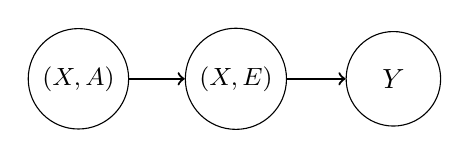
\begin{tikzpicture}

\node[circle,draw, minimum size=1.2cm] (R0) at (0,0) {\begin{small}$(X, A)$\end{small}
};
\node[circle,draw, minimum size=1.2cm] (R1) at (2,0) {\begin{small}$(X, E)$\end{small}};
\node[circle,draw, minimum size=1.2cm] (Y) at (4,0) {$Y$};

\path[->, thick] (R0) edge (R1);
\path[->, thick] (R1) edge (Y);

\end{tikzpicture}
\caption{Bayesian network corresponding to Assumption \ref{assum:indep-mips}.}
\label{fig:embedding_mips}
\vspace{-0.2cm}
%
\end{figure}


\myparagraph{Intuition}
The context-embedding pair $(X, E)$ can be seen as a representation of the context-action pair $(X, A)$ which contains less `redundant information' regarding the outcome $Y$. Intuitively, the MIPS estimator, which only considers the shift in the distribution of $(X, E)$ is therefore more efficient than the IPW estimator (which considers the shift in the distribution of $(X, A)$ instead). 
%

\myparagraph{MR achieves lower variance than MIPS}
Given the intuition above, we should achieve greater variance reduction as the amount of redundant information in the representation $(X, E)$ decreases. We formalise this in Appendix \ref{app:gmips} and show that the variance of MIPS estimator decreases as the representation gets closer to $Y$ in terms of information content. As a result, we achieve the greatest variance reduction by considering the marginal shift in the outcome $Y$ itself (as in MR) rather than the shift in the representation $(X, E)$ (as in MIPS). The following result formalizes this finding. 
%
%
\begin{theorem}\label{prop:mips_main_text}
    When the weights $w(y)$, $\frac{\ptar(e, x)}{\pbeh(e, x)}$ and $\rho(a, x)$ are known exactly, then under Assumption \ref{assum:indep-mips}, 
    \begin{align*}
        \Ebeh[\thetamr] = \Ebeh[\hat{\theta}_{\textup{MIPS}}] = \Etar[Y], \quad \textup{and} \quad \Vbeh[\thetamr] \leq \Vbeh[\hat{\theta}_{\textup{MIPS}}] \leq \Vbeh[\thetaipw].
    \end{align*}
    %
    %
    %
\end{theorem}
%
This analysis provides a link between the MR and MIPS estimators in the framework of contextual bandits, and shows that the MR estimator achieves lower variance than MIPS estimator while not requiring any additional assumptions (e.g.\ Assumption \ref{assum:indep-mips} as in MIPS). We also verify this empirically in Section \ref{sec:exp-synth} by reproducing the experimental setup in \cite{saito2022off} along with the MR baseline.
%

%

%

%

\subsubsection{Weight estimation error}\label{subsec:weight-estimation-error}
%
%
%
Our analysis so far assumes prior knowledge of the behavior policy $\beh$ and the marginal ratios $w(y)$. However, in practice, both quantities are often unknown and must be estimated from data. To this end, we assume access to an additional training dataset $\Dtr = \{(x^\tr_i, a^\tr_i, y^\tr_i)\}_{i=1}^m$ (for weight estimation), in addition to the evaluation dataset $\D = \{(x_i, a_i, y_i)\}_{i=1}^n$ (for computing the OPE estimate). 
%
%
The estimation of $\hat{w}(y)$ involves a two-step process that exclusively utilizes data from $\Dtr$:
%
%
\begin{enumerate}[label=(\roman*)]
    \item First, we estimate the policy ratio $\hat{\rho}(a, x) \approx \frac{\tar(a | x)}{\beh(a | x)}$. This can be achieved by estimating the behaviour policy $\hatbeh$, and defining $\hat{\rho}(a, x)\coloneqq \frac{\tar(a\mid x)}{\hatbeh(a\mid x)}$. Alternatively, $\hat{\rho}(a, x)$ can also be estimated directly by using density ratio estimation techniques as in \cite{sondhi2020balanced}.
    \item Secondly, we estimate the weights $\hat{w}(y)$ using Eq. \eqref{eq:weights-obj-main} with $\hat{\rho}$ instead of $\rho$.
\end{enumerate}

    %
    %
    %
    %
 
%
%
%

In practice, one may consider splitting $\Dtr$ for each estimation step outlined above. Moreover,
each approximation step may introduce bias and therefore, the MR estimator may have two sources of bias.
%
%
%
%
While classical OPE methods like IPW and DR also suffer from bias because of $\hat{\rho}$ estimation, the estimation of $\hat{w}(y)$ is specific to MR. However, we show below
that given any policy ratio estimate $\hat{\rho}$, if $\hat{w}(y)$ approximates $\Ebeh[\hat{\rho}(A, X)\mid Y=y]$ `well enough' (i.e., the estimation step (ii) shown above is `accurate enough'), 
then MR achieves a lower variance than IPW and incurs little extra bias.

\begin{proposition}\label{prop:bias-and-var-main}
Suppose that the IPW and MR estimators are defined as,
\[
\approxipw \coloneqq \frac{1}{n}\sum_{i=1}^n\hat{\rho}(a_i, x_i)\, y_i, \quad \textup{and }\quad \approxmr \coloneqq \frac{1}{n}\sum_{i=1}^n\hat{w}(y_i)\, y_i,
\]
and define the approximation error as $\epsilon \coloneqq \hat{w}(Y) - \tilde{w}(Y)$, where $\tilde{w}(Y) \coloneqq \Ebeh[\hat{\rho}(A, X)\mid Y]$. Then we have that, $\textup{Bias}(\approxmr) - \textup{Bias}(\approxipw) = \Ebeh[\epsilon\,Y]$. Moreover,
%
%
%
%
%
%
%
\begin{small}
\begin{align}
    \Vbeh[\approxipw] - \Vbeh[\approxmr]
    %
    &= \frac{1}{n}(\underbrace{\Ebeh[\Vbeh[\hat{\rho}(A, X)\,Y\mid Y]]}_{\geq 0} - \Vbeh[\epsilon\,Y] - 2\,\textup{Cov}(\tilde{w}(Y)\,Y, \epsilon\,Y)). \label{eq:var-difference-approximate-weights}
\end{align}
\end{small}
%
%
%
%
%
\end{proposition}
%
\myparagraph{Intuition} The $\epsilon$ term defined in Proposition \ref{prop:bias-and-var-main} denotes the error of the second approximation step outlined above. 
As a direct consequence of this result, we show in Appendix \ref{sec:wide_nns_weight_estimation} that as the error $\epsilon$ becomes small (specifically as $\Ebeh[\epsilon^2]\rightarrow 0$), the difference between biases of MR and IPW estimator becomes negligible.
%
Likewise, the terms $\Vbeh[\epsilon\,Y]$ and $\textup{Cov}(\tilde{w}(Y)\,Y, \epsilon\,Y)$ in Eq. \eqref{eq:var-difference-approximate-weights} will also be small and as a result the variance of MR will be lower than that of IPW (as the first term is positive). 

In fact, using recent results regarding the generalisation error of neural networks \citep{lai2023generalization}, we show that when using 2-layer wide neural networks to approximate the weights $\hat{w}(y)$, the estimation error $\epsilon$ declines with increasing training data size $m$. Specifically, under certain regularity assumptions we obtain $\Ebeh[\epsilon^2] = O(m^{-2/3})$. Using this we show that as the training data size $m$ increases, the biases of MR and IPW estimators become roughly equal with a high probability, and
\[
\Vbeh[\approxipw] - \Vbeh[\approxmr] = \frac{1}{n}\,\Ebeh[\Vbeh[\hat{\rho}(A, X)\,Y\mid Y]] + O(m^{-1/3}).
\]
Therefore the variance of MR estimator falls below that of IPW for large enough $m$. The empirical results shown in Appendix \ref{subsec:mips-empirical} are consistent with this result. Due to space constraints, the main technical result has been included in Appendix \ref{sec:wide_nns_weight_estimation}.

%
%

%
%
%

%
%
%
%
%
%
%
%
%
%
%
%
%
%
%
%
%
%
%
%
%
%
%
%

%
%
 
%
%
%
%
%

\subsection{Application to causal inference}\label{subsec:application-to-causal-inference}
 Beyond contextual bandits, the variance reduction properties of the MR estimator make it highly useful in a wide variety of other applications. Here, we show one such application in the field of causal inference, where MR can be used for the estimation of average treatment effect (ATE) \citep{pearl2009causality} and leads to some desirable properties in comparison to the conventional ATE estimation approaches. Specifically, we illustrate that the MR estimator for ATE utilizes the evaluation data $\D$ more efficiently and achieves lower variance than state-of-the-art ATE estimators and consequently provides more accurate ATE estimates.
%
%
%
%
To be concrete, the goal in this setting is to estimate ATE, defined as follows:
%
\[
\ate \coloneqq \E[Y(1)-Y(0)].
\]
Here $Y(a)$ corresponds to the outcome under a deterministic policy $\pi_a(a'\mid x) \coloneqq \ind(a'=a)$. Hence any OPE estimator can be used to estimate $\E[Y(a)]$ (and therefore ATE) by considering target policy $\tar = \pi_a$.
%
%
%
An important distinction between MR and existing approaches (like IPW or DR) is that, when estimating $\E[Y(a)]$, the existing approaches only use datapoints in $\D$ with $A=a$. To see why this is the case, we note that the policy ratios $\frac{\tar(A|X)}{\beh(A|X)} = \frac{\ind(A=a)}{\beh(A|X)}$ are zero when $A\neq a$. In contrast, the MR weights $\frac{\ptar(Y)}{\pbeh(Y)}$ are not necessarily zero for datapoints with $A\neq a$, and therefore the MR estimator uses all evaluation datapoints when estimating $\E[Y(a)]$. 

As such we show that MR applied to ATE estimation leads to a smaller variance than the existing approaches. Moreover, because MR is able to use all datapoints when estimating $\E[Y(a)]$, MR will generally be more accurate than the existing methods especially in the setting where the data is imbalanced, i.e., the number of datapoints with $A=a$ is small for a specific action $a$.
In Appendix \ref{app:causal-inference}, we formalise this variance reduction of the MR ATE estimator compared to IPW and DR estimators, by deriving analogous results to Propositions \ref{prop:var_mr} and \ref{prop:var_dr}. In addition, we also show empirically in Section \ref{subsec:causal-experiments} that the MR ATE estimator outperforms the most commonly used ATE estimators.
\begin{comment}

\begin{proposition}\label{prop:bias-and-var}
Let 
\[
\thetaipw = \frac{1}{n}\hat{\rho}(a_i, x_i)\, y_i,
\]
where $\hat{\rho}(a, x)\coloneqq \tar(a\mid x)/\hatbeh(a\mid x)$. Additionally, let
\[
\thetamr = \frac{1}{n}\hat{w}(y_i)\, y_i,
\]
where $\hat{w}(y)$ satisfies Eq. $\eqref{eq:estimated-marginal-ratio}$. Then, 
\begin{align*}
    \textup{Bias}(\thetamr) &= \textup{Bias}(\thetaipw) \qquad \textup{and,} \\
    n (\Vbeh[\thetaipw] - \Vbeh[\thetamr]) 
    &= \E_{Y\sim \pbeh(Y)} \left[ \Vbeh\left[ \hat{\rho}(A, X) \mid Y \right]\, Y^2 \right].
\end{align*}
\end{proposition}
More generally, if $\hat{w}$ is a `noisy' estimate of the conditional expectation $\Ebeh[\hat{\rho}(A, X)\mid Y]$, we can obtain similar results regarding the bias and variance of the MR estimators under certain assumptions. 
\end{comment}


%

%

%



\begin{comment}
    

Specifically, the traditional IPW estimator applied to ATE estimation yields:
\[
\ateipw = \frac{1}{n} \sum_{i=1}^n \rho_{\ate}(a_i, x_i) \times y_i, \qquad \textup{where, } \qquad \rho_{\ate}(a, x) \coloneqq \frac{\mathbbm{1}(a=1) - \mathbbm{1}(a=0)}{\beh (a|x)}.
\]

Simlarly, the MR estimator can be written as
$$
\atemr = \frac{1}{n}\sum_{i=1}^n w_{\ate}(y_i)\times y_i, \qquad \textup{where, } \qquad w_{\ate}(y) = \frac{p_{\pi^{(1)}}(y) - p_{\pi^{(0)}}(y)}{\pbeh(y)},
$$ 
and $\pi^{(a)}(a'\mid x) \coloneqq \mathbbm{1}(a'=a)$ for $a\in \{0,1\}$, and $w_{\ate}(y)$ can be estimated using regression similar to Eq. \eqref{eq:weights-obj-main}.
\end{comment}
%
%
%
%

%
%
%
%
%
%
%
%
%
%
%
%
%
%
%
%
%
%
%



\subsection{Plasticity in Neural Networks}
In recent years, various methods have been proposed to address plasticity loss.
Several works have focused on maintaining active units \cite{abbas2023loss, elsayed2024addressing} or re-initializing dead units \cite{sokar2023dormant, dohare2024loss}.
Other studies have explored limiting deviations from the initial statistics of model parameters \cite{kumar2023maintaining, lewandowski2023curvature, elsayed2024weight}.
Additionally, some methods rely on architectural modifications \cite{nikishin2024deep, lee2024slow, lewandowski2024plastic}.  
Plasticity loss also occurs in the reinforcement learning due to its inherent non-stationary. \citet{nikishin2022primacy} proposed resetting the model, while \citet{asadi2024resetting} suggested resetting the optimizer state. 

As noted by \citet{berariu2021study}, loss of plasticity can be divided into two distinct aspects: a decreased ability of networks to minimize training loss on new data (trainability) and a decreased ability to generalize to unseen data (generalizability).
While most previous works focused on trainability, \citet{lee2024slow} addressed generalizability loss.
They demonstrated that plasticity loss also occurs under a stationary distribution, as in a warm-start learning scenario where the model is pretrained on a subset of the training data and then fine-tuned on the full dataset.

Most existing studies have focused on only one of the following challenges: trainability, generalizability, or reinforcement learning.
However, in this study, we validate our AID method across all three aspects, demonstrating its effectiveness in each scenario.



\subsection{Activation Function}
Our AID method is a stochastic approach similar to Dropout while also functioning as an activation function.
Therefore, we aim to discuss previously proposed probabilistic activation functions.
Although the field of probabilistic activation functions has not seen extensive research, two noteworthy studies exist.
The first is the Randomized ReLU (RReLU) function, introduced in the Kaggle NDSB Competition \cite{xu2015empirical}.
The original ReLU function maps all negative values to zero, whereas RReLU maps negative values linearly based on a random slope.
During testing, negative values are mapped using the mean of the slope distribution.
Their experimental results suggest that RReLU effectively prevents overfitting.
Another example of a probabilistic activation function is DropReLU \cite{liang2021drop}.
DropReLU randomly determines whether a node's activation is processed through a ReLU function or a linear function.
The authors claim that DropReLU improves the generalization performance of neural networks.
The fundamental distinction between these probabilistic activation functions and our method lies in the generality of our approach.
Unlike simple probabilistic activation functions, our method encompasses techniques such as Dropout and ReLU, providing a more comprehensive framework.

Another related approach involves activation functions designed to address plasticity loss.
\citep{abbas2023loss} proposed the Concatenated Rectified Linear Units (CReLU), which concatenates the outputs of the standard ReLU applied to the input and its negation.
This structure prevents the occurrence of dead units, thereby improving plasticity.
Additionally, trainable activation functions have also been shown to effectively mitigate plasticity loss in reinforcement learning \citep{delfosseadaptive}.
Specifically, they introduced a trainable rational activation function that prevents value overfitting and overestimation in reinforcement learning.



\begin{figure*}[ht!]
    \centering
    \includegraphics[width=0.3\textwidth]{figures/sources/mainnet_pls_acc.pdf}
    \includegraphics[width=0.3\textwidth]{figures/sources/subnet_pls_acc.pdf}
    \includegraphics[width=0.3\textwidth]{figures/sources/warm_start_dropout.pdf}
    \caption{\textbf{Left.} Random label MNIST experiment using an 8-layer MLP. Higher dropout probabilities result in significant trainability loss. 
    \textbf{Middle.} Accuracy of the subnetworks trained on random target. Each subnetworks are sampled from original network after each epoch. Subnetworks of the Dropout also experience trainability loss. \textbf{Right.} Warm-start scenario of Resnet-18 model with CIFAR100 dataset. Dropout improves generalization performance; however, the reduction in accuracy compared to the cold-start scenario is nearly identical to that of the vanilla model.}
    \label{exp_dropout}
\end{figure*}




\section{Empirical evaluation}
In this section, we provide empirical evidence to support our theoretical results by investigating the performance of our MR estimator against the current state-of-the-art OPE methods. The code to reproduce our experiments has been made available at: \href{https://github.com/faaizT/MR-OPE}{\textcolor{blue}{github.com/faaizT/MR-OPE}}.
%
%
%
%
%
%

\subsection{Experiments on synthetic data}\label{sec:exp-synth}
For our synthetic data experiment, we reproduce the experimental setup for the synthetic data experiment in \cite{saito2022off} by reusing their code with minor modifications.
%
Specifically, $\Xspace \subseteq \mathbb{R}^d$, for various values of $d$ as described below. Likewise, the action space $\Aspace = \{0, \dots, n_a-1\}$, with $n_a$ taking a range of different values. Additional details regarding the reward function, behaviour policy $\beh$, and the estimation of weights $\hat{w}(y)$ have been included in Appendix \ref{subsec:mips-empirical} for completeness. 

%
%


\myparagraph{Target policies} 
To investigate the effect of increasing policy shift, we define a class of policies,
\[
%
\pi^{\alpha^\ast}(a | x) = \alpha^\ast\,\ind(a = \arg\max_{a'\in \Aspace} q(x, a')) + \frac{1-\alpha^\ast}{|\Aspace|} \quad \textup{where} \quad q(x, a) \coloneqq \E[Y\mid X=x, A=a],
%
\]
where $\alpha^\ast \in [0, 1]$ allows us to control the shift between $\beh$ and $\tar$. In particular, as we show later, the shift between $\beh$ and $\tar$ increases as $\alpha^\ast \rightarrow 1$. Using the ground truth behaviour policy $\beh$, we generate a dataset which is split into training and evaluation datasets of sizes $m$ and $n$ respectively. 


%
%
%
%
%
%
%
%
%
%

%
%
%
%
%

%
%
%
%
%
%
%


\myparagraph{Baselines} 
We compare our estimator with DM, IPW, DR and MIPS estimators. Our setup includes action embeddings $E$ satisfying Assumption \ref{assum:indep-mips}, and so MIPS is unbiased.
%
%
Additional baselines have been considered in Appendix \ref{subsec:mips-empirical}.
For MR, we split the training data to estimate $\hatbeh$ and $\hat{w}(y)$, whereas for all other baselines we use the entire training data to estimate $\hatbeh$ for a fair comparison.
%
%
%
%
\begin{figure}[t]
     \centering
     \begin{subfigure}[b]{0.5\textwidth}
         \centering
         \includegraphics[height=1.06in]{figures/mr/ope_vs_neval_nac_100_alphatar_0_8_dimc_1000_untrunc.png}
         \caption{Results with varying evaluation data size $n$.}
         \label{fig:mse-vs-neval}
     \end{subfigure}%
     \begin{subfigure}[b]{0.5\textwidth}
         \centering
         \includegraphics[height=1.06in]{figures/mr/ope_vs_alphatar_nac_100_neval_800_dimc_1000.png}
         \caption{Results with varying $\alpha^\ast$.}
         \label{fig:mse-vs-betatar}
     \end{subfigure}\\
    \caption{Results for synthetic data experiment. In \ref{fig:mse-vs-neval} we have $\alpha^\ast=0.8$ and in \ref{fig:mse-vs-betatar} we have $n = 800$.}
    \label{fig:syn_results1}
\end{figure}

%
%
%
%
%
%
%
%
%
%
%
%
%
%
%
%
%
\myparagraph{Results}
We compute the target policy value using the $n$ evaluation datapoints. Here, the MSE of the estimators is computed over 10 different sets of logged data replicated with different seeds. The results presented have context dimension $d=1000$, number of actions $n_a=100$ and training data size $m=5000$. More experiments for a variety of parameter values are included in Appendix \ref{subsec:mips-empirical}.


%
%
%
%
%
%
%
%
%
%
%
%
%
%
%
%
%
%
%
%
%
%
%
%
%
%
%
%
%

\myparagraph{Varying number of evaluation data $n$} 
In Figure \ref{fig:mse-vs-neval} we plot the results with increasing size of evaluation data $n$ increases. MR achieves the smallest MSE among all the baselines considered when $n$ is small, with the MSE of MR being at least an order of magnitude smaller than every baseline for $n\leq 500$. This shows that MR is significantly more accurate than the baselines when the size of the evaluation data is small. As $n\rightarrow \infty$, the difference between the results for MR and MIPS decreases. However, MR attains smaller variance and MSE than MIPS generally, verifying our analysis in Section \ref{subsec:mips-comparison}.
%
%
%
Moreover, Figure \ref{fig:mse-vs-neval} shows that while the variance of MR is greater than that of DM, it still achieves the lowest MSE overall, owing to the high bias of DM.

\begin{wrapfigure}{r}{0.35\textwidth}
    \centering
    \includegraphics[width=0.35\textwidth]{figures/mr/kl-divergence-w-uncertainty.png}
    %
    %
    %
\end{wrapfigure}
\myparagraph{Varying $\alpha^\ast$}
As $\alpha^\ast$ parameter of the target policy increases, so does the shift between the policies $\beh$ and $\pi^{\alpha^\ast}$ as illustrated by the figure on the right, which plots the KL-divergence $D_{\textup{KL}}(\beh\, || \, \pi^{\alpha^\ast})$ as a function of $\alpha$.
%
%
%
Figure \ref{fig:mse-vs-betatar} plots the results for increasing policy shift. 
Overall, the MSE of MR estimator is lowest among all the baselines. Moreover, while the MSE and variance of all estimators increase with increasing $\alpha^\ast$ the increase in these quantities is lower for the MR estimator than for the other baselines. Therefore, the relative performance of MR estimator improves with increasing policy shift and MR remains robust to increase in policy shift.
%
%
%

\myparagraph{Additional ablation studies}
In Appendix \ref{subsec:mips-empirical}, we investigate the effect of varying context dimensions $d$, number of actions $n_a$ and number of training data $m$. In every case, we observe that the MR estimator has a smaller MSE than all other baselines considered. In particular, MR remains robust to increasing $n_a$ whereas the MSE and variance of IPW and DR estimators degrade substantially when $n_a \geq 2000$. Likewise, MR outperforms the baselines even when the training data size $m$ is small.

%
%
%
%
%
%
%
%
%
%
%
%
%
%
%
%
%
%
%
%
%
%
%
%
%
%
%
%
%
%
%
%
%
%
%
%
%
%
%
%
%
%
%
%
%
%
%
%
%
%
%
%
%
%
%
%
\begin{sidewaystable}[!htp]
    \centering
    \caption{Mean squared error of target policy value with standard errors over 10 different seeds for different classification datasets. Here, number of evaluation data $n=1000$, and $\alpha^\ast=0.6$.}
    \label{tab:classification-dataset-results}
    \begin{footnotesize}
    \begin{scshape}
%
%
%
%
%
%
%
%
%
%
%
%

\begin{tabular}{llllllll}
\toprule
Dataset &             Digits &               Letter &          OptDigits &          PenDigits &           SatImage  &              Mnist & CIFAR-100\\
\midrule
DM        &  0.1508$\pm$0.0015 &    0.0886$\pm$0.0026 &  0.0485$\pm$0.0016 &   0.0520$\pm$0.0016 &  0.0208$\pm$0.0009  &  0.1109$\pm$0.0014 & 0.0020$\pm$0.0001 \\
DR        &    0.1334$\pm$0.0400 &    \red{35.085$\pm$17.768} &  0.0464$\pm$0.0061 &  0.2343$\pm$0.1404 &   0.0560$\pm$0.0395 &  0.2617$\pm$0.0139 & \red{3823.9$\pm$2023.2} \\
DRos      &  0.0847$\pm$0.0025 &    0.2363$\pm$0.0586 &  0.0384$\pm$0.0025 &  0.0138$\pm$0.0029 &  0.0078$\pm$0.0008 &  0.2151$\pm$0.0061 & 0.2628$\pm$0.1087 \\
IPW       &  0.1632$\pm$0.0462 &  \red{45.253$\pm$22.057} &   0.0844$\pm$0.0056 &  0.1342$\pm$0.0531 &    0.0900$\pm$0.0676 & 0.3359$\pm$0.0118 & \red{4116.9$\pm$2097.9}\\
SwitchDR  &  0.0982$\pm$0.0032 &    0.2387$\pm$0.0507 &  0.0557$\pm$0.0047 &   0.0342$\pm$0.0090 &  0.0136$\pm$0.0012  &   0.2750$\pm$0.0102 & 1.1644$\pm$0.8227 \\
MR (Ours) &  \textbf{0.0034$\pm$0.0001} &    \textbf{0.0018$\pm$0.0004} &  \textbf{0.0006$\pm$0.0002} &  \textbf{0.0008$\pm$0.0002} &  \textbf{0.0016$\pm$0.0003} &  \textbf{0.0121$\pm$0.0009} &  \textbf{0.0007$\pm$0.0002}\\
\bottomrule
\end{tabular}

%
%
%
%
%
%
%
%
%
%
%
%
\end{scshape}
\end{footnotesize}
\end{sidewaystable}
\subsection{Experiments on classification datasets}
Following previous works on OPE in contextual bandits \citep{dudik2014doubly, kallus2021optimal, mehrdad2018more,wang2017optimal}, we transform classification datasets into contextual bandit feedback data in this experiment.
We consider five UCI classification datasets \citep{dua2019uci} as well as Mnist \citep{deng2012mnist} and CIFAR-100 \citep{krizhevsky2009learning} datasets, each of which comprises $\{(x_i, a^\gt_i)\}_{i}$, where $x_i\in \Xspace$ are feature vectors and $a^\gt_i\in \Aspace$ are the ground-truth labels.
%
%
In the contextual bandits setup, the feature vectors $x_i$ are considered to be the contexts, whereas the actions correspond to the possible class of labels. For the context vector $x_i$ and the action $a_i$, the reward $y_i$ is defined as $y_i \coloneqq \ind(a_i = a^\gt_i)$, i.e., the reward is 1 when the action is the same as the ground truth label and 0 otherwise. Here, the baselines considered include the DM, IPW and DR estimators as well as Switch-DR \citep{wang2017optimal} and DR with Optimistic Shrinkage (DRos) \citep{su2020doubly}. We do not consider a MIPS baseline here as there is no natural embedding $E$ of $A$. Additional details are provided in Appendix \ref{subsec:additional-experiments-classification}. 
%
%
%

In Table \ref{tab:classification-dataset-results}, we present the results with number of evaluation data $n=1000$ and number of training data $m=500$. 
The table shows that across all datasets, MR achieves the lowest MSE among all methods. \flag{Moreover, for the Letter and CIFAR-100 datasets the IPW and DR yield large bias and variance arising from poor policy estimates $\hatbeh$. Despite this, the MR estimator which utilizes the \emph{same} $\hatbeh$ for the estimation of $\hat{w}(y)$ leads to much more accurate results.} We also verify that MR outperforms the baselines for increasing policy shift and evaluation data $n$ in Appendix \ref{subsec:additional-experiments-classification}.
%


%

%

%
%
%
%
%

\subsection{Application to ATE estimation}\label{subsec:causal-experiments}
%
In this experiment, we investigate the empirical performance of the MR estimator for ATE estimation. 

\myparagraph{Twins dataset}
We use the Twins dataset studied in \cite{louizos2017causal}, which comprises data from twin births in the USA between 1989-1991. The treatment $a=1$ corresponds to being born the heavier twin and the outcome $Y$ corresponds to the mortality of each of the twins in their first year of life. Specifically, $Y(1)$ corresponds to the mortality of the heavier twin (and likewise for $Y(0)$). To simulate the observational study, we follow a similar strategy as in \cite{louizos2017causal} to selectively hide one of the two twins as explained in Appendix \ref{app:ate-empirical}. We obtain a total of 11,984 datapoints, of which 5000 datapoints are used to train the behaviour policy $\hatbeh$ and outcome model $\hat{q}(x, a)$.

%
%

%
\begin{table}[t]
%
    \centering
    \caption{Mean absolute ATE estimation error $\epsilon_\ate$ with standard errors over 10 different seeds, for increasing number of evaluation data $n$.}
    \label{tab:ate_errors-main}
    \begin{small}
    \begin{tabular}{lllll}
\toprule
$n$ &             50   &             200  &             1600 &             3200 \\
\midrule
DM       &  0.092$\pm$0.003 &  0.092$\pm$0.003 &  0.092$\pm$0.004 &  0.092$\pm$0.004 \\
DR       &  0.101$\pm$0.024 &  \textbf{0.065$\pm$0.009} &  0.071$\pm$0.005 &  0.069$\pm$0.004 \\
\textsc{DRos}     &    0.100$\pm$0.017 &  0.089$\pm$0.006 &   0.093$\pm$0.004 &  0.087$\pm$0.004 \\
IPW      &  0.092$\pm$0.024 &  0.088$\pm$0.014 &  0.067$\pm$0.007 &  0.067$\pm$0.007 \\
\textsc{SwitchDR} &  0.101$\pm$0.024 &  \textbf{0.065$\pm$0.009} &  0.071$\pm$0.005 &  0.069$\pm$0.004 \\
MR (Ours)      &  \textbf{0.062$\pm$0.007} &  \textbf{0.065$\pm$0.007} &  \textbf{0.061$\pm$0.005} &  \textbf{0.061$\pm$0.006} \\
\bottomrule
\end{tabular}
\end{small}
%
\end{table}
%
Here, we consider the same baselines as the classification data experiments in previous section.
For our evaluation, we consider the absolute error in ATE estimation, $\epsilon_\ate$, defined as:
$
\epsilon_\ate \coloneqq | \hat{\theta}^{(n)}_\ate - \theta_\ate |.
$
Here, $\hat{\theta}^{(n)}_\ate$ denotes the value of the ATE estimated using $n$ evaluation datapoints.
%
We compute the ATE value using the $n$ evaluation datapoints, over 10 different sets of observational data (using different seeds). Table \ref{tab:ate_errors-main} shows that MR achieves the lowest estimation error $\epsilon_\ate$ for all values of $n$ considered here. While the performance of other baselines improves with increasing $n$, MR outperforms them all. 
%


%
%
%
%
%
%
%
%
%
%
%
%
%
%
%
%
%
%
%


%
%
%

%
%

This work identifies signal collapse as a critical bottleneck in one-shot neural network pruning. Performance loss in pruned networks is due to \textbf{signal collapse} in addition to the removal of critical parameters. We propose \textbf{REFLOW} (\textbf{Re}storing \textbf{F}low of \textbf{Low}-variance signals), a simple yet effective method that mitigates signal collapse without computationally expensive weight updates. By focusing on signal preservation, REFLOW highlights the importance of mitigating signal collapse in sparse networks and enables magnitude pruning to match or surpass state-of-the-art one-shot pruning methods such as CHITA, CBS, and WF.

REFLOW consistently achieves state-of-the-art accuracy across diverse architectures, restoring ResNeXt-101 from under 4.1\% to 78.9\% top-1 accuracy at 80\% sparsity on ImageNet. Its lightweight design makes it a practical solution for both research and deployment, delivering high-quality sparse models without the overhead of traditional approaches. These findings challenge the traditional emphasis on weight selection strategies and underscore the critical role of signal propagation for achieving high-quality sparse networks in the context of one-shot pruning.


